\documentclass[a4paper, 12pt]{article}

% Работа с русским языком
\usepackage{cmap}
\usepackage{mathtext}
\usepackage[T2A]{fontenc}
\usepackage[utf8]{inputenc}
\usepackage[english,russian]{babel}

% Математика и графика
\usepackage{amsmath,amsfonts,amssymb,amsthm,mathtools}
\usepackage{icomma}

\usepackage{physics}
\usepackage{graphicx}
\usepackage{calc}
\usepackage{wrapfig}
\usepackage{setspace}
\usepackage{indentfirst}
\usepackage{gensymb}
\usepackage{longtable}
\usepackage{float}
\usepackage{multirow}

\usepackage{amsmath} % Для математических формул
\usepackage{amssymb} % Для математических символов
\usepackage{tikz} % Для графиков
\usepackage{wrapfig} % Для обтекания текста вокруг фигур

\setlength{\textfloatsep}{10pt}

% Точка после секции
\usepackage{titlesec}
\titlelabel{\thetitle.\quad}

\usepackage[left=25mm, top=14mm, right=25mm, bottom=30mm, nohead]{geometry}
\usepackage{fancybox,fancyhdr} 
\setcounter{page}{1} % счетчик нумерации страниц
\headsep=10mm 
\usepackage{xcolor}
\usepackage{hyperref} 
\hypersetup{colorlinks=true, allcolors=[RGB]{010 090 200}} % цвет ссылок 
\newcommand{\lr}[1]{\left({#1}\right)} % команда для скобок
\newcommand{\te}[2]{{#1}_{\text{#2}}}



\begin{document}

\begin{titlepage}
	\begin{center}
		\large 	Московский физико-технический институт \\
		Факультет общей и прикладной физики \\
		\vspace{0.2cm}
		
		\vspace{4.5cm}
		Лабораторная работа № 3.2.3\\ \vspace{0.2cm}
		\large (Общая физика: электричество и магнетизм) \\ \vspace{0.2cm}
		\LARGE \textbf{Резонанс токов в параллельном контуре}
	\end{center}
	\vspace{2.3cm} \large
	
	\begin{center}
		Работу выполнил: \\
		Комкин Михаил,
		Б01-303
		\vspace{10mm}		
		
	\end{center}
	
	\begin{center} \vspace{60mm}
		г. Долгопрудный \\
		2024 год
	\end{center}
\end{titlepage}



\paragraph*{Цель работы:} исследование резонанса токов в параллельном колебательном контуре с изменяемой
ёмкостью, включающее получение амплитудно-частотных и фазово-частотных характеристик, а также определение основных параметров контура.

\paragraph*{Оборудование:} генератор сигналов, источник тока, нагруженный на параллельный колебательный контур с переменной ёмкостью, двулучевой осциллограф, цифровые вольтметры.


\section{Теоретическое введение и описание установки}
\begin{figure}[h]
\begin{minipage}[h]{0.49\linewidth}
\center{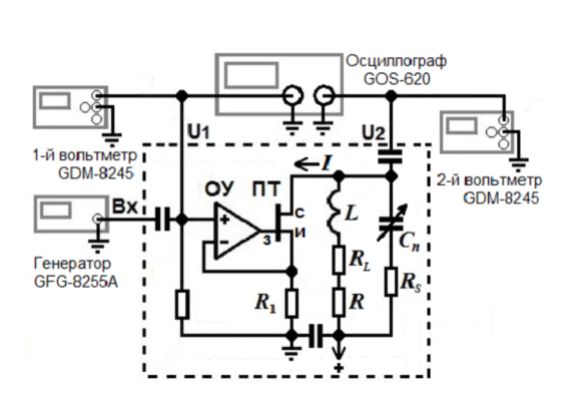
\includegraphics[width=1\linewidth]{im1.png} \\ Рис.1 Схема установки.}
\end{minipage}
\hfill
\begin{minipage}[h]{0.49\linewidth}
\center{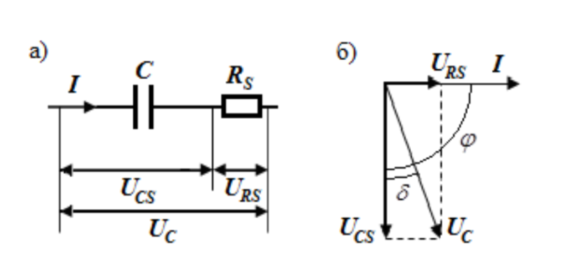
\includegraphics[width=1\linewidth]{im2.png} \\ Рис.2 Последовательная эквивалентная схема конденсатора с потерями.}
\end{minipage}
\end{figure}

$I=\dfrac{E}{R_I}=\dfrac{E_0cos(\omega t+\varphi_0)}{R_I}=I_0cos(\omega t+\varphi_0)$ --- ток на генераторе\newline
$$R_S=\dfrac{U_{RS}}{I}=\frac{U_{RS}}{\omega CU_{CS}}=\dfrac{1}{\omega C}tg\delta$$
где $R_S$ - эквивалентное последовательное сопротивление (ЭПС)\newline
Для используемых емкостей $C_n$ выполнено $tg\delta<10^{-3}$\newline
$$R_{\sum}=R+R_L+R_S$$
где $R_{\sum}$ - суммарное активное сопротивление контура.\newline
Воспользуемся методом комплексных амплитуд:\newline
$Z_L=R_L+i\omega L$, $Z_C=R_S-i\frac{1}{\omega C}$, $Z=R_{\sum}+i(\omega L-d\dfrac{1}{\omega C})$\newline
Тогда напряжение на контуре и токи на индуктивной и емкостной частях контура при нулевой начальной фазе можно предствить в виде:\newline
$$I_c=I\dfrac{Z_L}{Z_C+Z_L}=iQI_0\dfrac{\omega}{\omega_0}\dfrac{1-i\dfrac{R+R_L}{\rho}\dfrac{\omega_0}{\omega}}{1+iQ(\dfrac{\omega}{\omega_0}-\dfrac{\omega_0}{\omega})}$$
$$I_L=I\dfrac{Z_c}{Z_C+Z_L}=iQI_0\frac{\omega_0}{\omega}\frac{1+itg\delta}{1+iQ(\frac{\omega}{\omega_0}-\frac{\omega_0}{\omega})}$$
$$U=I\frac{Z_LZ_c}{Z_C+Z_L}=Q\rho I_0\frac{(1-i\frac{R+R_L}{\rho}\frac{\omega_0}{\omega})(1+itg\delta)}{1+iQ(\frac{\omega}{\omega_0}-\frac{\omega_0}{\omega})}$$
где $\omega_0=\frac{1}{\sqrt{LC}}$ - собственная частота, $\rho=\sqrt{\frac{L}{C}}$ - реактивное сопротивление контура, $Q=\frac{\rho} - {R_{\sum}}$ - добротность контура\newline
Рассмотрим случай, когда $|\Delta\omega|=|\omega-\omega_0|\ll\omega_0$. Тогда
$$\frac{\omega}{\omega_0}-\frac{\omega_0}{\omega}=\frac{2\Delta\omega}{\omega_0}$$
Пренебрегая поправками порядка $Q^{-2}$, получим:
$$I_c=QI_0\frac{\omega}{\omega_0}\frac{e^{i\phi_c}}{\sqrt{1+(\tau\Delta\omega)^2}},    \phi_c=\frac{\pi}{2}-\frac{R+R_L}{\rho}-arctg(\tau\Delta\omega)$$
$$I_L=QI_0\frac{\omega_0}{\omega}\frac{e^{i\phi_L}}{\sqrt{1+(\tau\Delta\omega)^2}}, \phi_L=-\frac{\pi}{2}+\delta\arctg(\tau\Delta\omega)$$
$$U=Q\rho I_0\frac{\omega}{\omega_0}\frac{e^{i\phi_U}}{\sqrt{1+(\tau\Delta\omega)^2}}, \phi_U=-\frac{\omega}{\omega_0}\frac{R+R_L}{\rho}+\delta-arctg(\tau\Delta\omega)$$
где $\tau=\frac{2L}{R_{\sum}}=\frac{2Q}{\omega_0}$ - время затухания.\newline
При резонансе, т.е. когда $\Delta\omega=0$:
$$I_c(\omega_0)=QI_0, \phi_c(\omega_0)=\frac{\pi}{2}-\frac{R+R_L}{\rho}$$
$$I_L(\omega_0)=QI_0, \phi_L(\omega_0)=-\frac{\pi}{2}+\delta$$
$$U(\omega_0)=Q\rho I_0=Q^2R_{\sum}I_0, \phi_U{\omega_0}=-\frac{R+R_L}{\rho}+\delta$$
$$\phi'_c(\omega_0)=\phi'_L(\omega_0)=\phi'_U(\omega_0)=-\tau$$
\section{Ход работы}

Данные установки: $ R = 3,50  $ Ом, $ R_1 = 1008 $ Ом.

\subsection{Измерения резонансных частот и напряжений, а также сопутствующих величин}

Проведем для 7 разных конденсаторов емкости $ C_n $ измерения резонансных частот и напряжений на них, поддерживая напряжение на вольтметре 1 равным $ E = 0,2 $ В, а также вычислим дополнительные величины, следующие из наших измерений, по следующим формулам:  

\begin{equation}\label{}
L=\frac{1}{C(2\pi f)^2} \\
\end{equation}
\begin{equation}\label{}
\rho=\frac{1}{2\pi fC} \\
\end{equation}
\begin{equation}\label{}
Z_{\text{рез}}=\frac{U}{E_0}R_1
\end{equation}
\begin{equation}\label{}
Q=\frac{UR_1}{E_0}2\pi fC
\end{equation}
\begin{equation}\label{}
R_{\sum}=\frac{E_0}{UR_1}\frac{1}{(2\pi fC)^2}
\end{equation}
\begin{equation}\label{}
R_{Smax}=10^{-3}\cdot\frac{1}{\omega_0C}
\end{equation}
\begin{equation}\label{}
R_L=\frac{E_0}{UR_1}\frac{1}{(2\pi fC)^2}-R-10^{-3}\cdot\frac{1}{\omega_0C}
\end{equation}

Результаты занесём в таблицу: 

\begin{table}[h!]
	\centering
	\caption{Результаты измерений при $ E = 0,2 \; Ом $}
\begin{tabular}{|c|c|c|c|c|c|c|c|c|c|c|}
	\hline
	$ C_n, нФ $ & $ f_{0n} $, кГц & $ U_{0n}, $ B & $ E $, B & $ L $, мкГн & $ \rho $, Ом & $ Z_{рез} $, Ом & $ Q $ & $ R_\Sigma,  $ Ом & $ R_{Sm} $, Ом & $ R_L $, Ом \\
	\hline
25.1 & 32.1 & 1.18 & 0.2 & 980.4 & 197.6 & 5947.2 & 30.1 & 6.57 & 0.20 & 2.9 \\
33.2 & 27.8 & 0.91 & 0.2 & 988.2 & 172.5 & 4586.4 & 26.6 & 6.49 & 0.17 & 2.8 \\
47.3 & 23.2 & 0.67 & 0.2 & 996.0 & 145.1 & 3376.8 & 23.3 & 6.24 & 0.15 & 2.6 \\
57.4 & 21.3 & 0.57 & 0.2 & 973.7 & 130.2 & 2872.8 & 22.1 & 5.90 & 0.13 & 2.3 \\
67.5 & 19.5 & 0.48 & 0.2 & 987.9 & 121.0 & 2419.2 & 20.0 & 6.05 & 0.12 & 2.4 \\
82.7 & 17.7 & 0.40 & 0.2 & 978.7 & 108.8 & 2016.0 & 18.5 & 5.87 & 0.11 & 2.3 \\
101.6 & 16.0 & 0.34 & 0.2 & 974.9 & 98.0 & 1713.6 & 17.5 & 5.60 & 0.10 & 2.0 \\
	\hline
	\multicolumn{4}{|c|}{Среднее значение} & 982,8 & & & & & & 2,5\\
	\multicolumn{4}{|c|}{Cлучайная погрешность} & 6,3 & & & & & & 0,2\\
	\hline
\end{tabular}
	\label{resC1}% 
\end{table}% 
\section{Измерение АЧХ}


По результатам построим графики АЧХ для обоих емкостей $C$


Проведем нормировку $U$ и $f$

Теперь найдем добротность по ширине резонансной кривой $ \delta\omega $ на 2 графике как 

\begin{equation}\label{}
Q = \dfrac{1}{\delta\omega}
\end{equation}  

Где $ \delta\omega $ --- расстояние между частотами при значении напряжения $ \dfrac{1}{\sqrt{2}} $.

Получаем ответ: 

\begin{equation}\label{}
Q_2 = 25,9 \pm 2 \qquad Q_5 = 19,7 \pm 2
\end{equation}
\subsection{Фазово-частотная характеристика}
Для тех же кондесаторов определим фазово-частотную характеристику. Будем определять разность фаз между сигналами $ U(t), E(t) $ как $ \Delta\phi = \dfrac{x}{x_0}\phi $, где $ x, x_0 $ --- расстояния от начала отсчёта до момента обращения графиков этих значений в нуль. Результаты занесем в таблицу:


Аналогично определим добротность, подсчитав длину резонансной кривой как  расстояние между частотами при разности фаз в $ \dfrac{3}{4}\pi $ и $ \dfrac{5}{4}\pi $:

\begin{equation}\label{}
Q_2 = 20,4 \pm 3\qquad Q_5 = 27,1 \pm 3
\end{equation}

\subsection{График  зависимости $ R_L $ от $ f_{0n} $} 

Теперь построим график зависимости $ R_L (f_{0n}) $ и проведем прямую $ \langle R_L \rangle = 2,5 $ Ом. 


 
Видно, что $ R_L$ возрастает при увеличении частоты. Это может быть объяснено скин-эффектом. 

Теперь построим векторную диаграмму для контура с наименьшей добротностью, т.е. для последнего --- $ Q_7 = 17,5 $. 

\begin{wrapfigure}{l}{0.34\linewidth} 
	\begin{tikzpicture} [scale = 1.8, yshift=2pt]
		\draw  (0, 0) -- (0, 2.1);
		\draw (0, 0) -- (0, - 2.1);
		\draw  (0, 0) -- (2.5, 0);
		\draw [->] (0, 0) -- (0.75, 2) node[anchor=west] {$ \vec{I_C} $};
		\draw (0, 1.3) arc (60:0: 0.6);
			\draw (0.2,1.4) node {$ \phi_C'$};
				\draw [->] (0, 0) -- (0.06, -2) node[anchor=west] {$ \vec{I_L} $};
			\draw (0, -1.3) arc (0:30: -0.4);
			\draw (0.15,-1.4) node {$ \delta$};
			\draw [->] (0, 0) -- (0.75, 0) node[anchor=south] {$ \vec{I} $};
			\draw [->] (0, 0) -- (1.75, -0.4) node[anchor=north] {$ \vec{U} $};
				\draw (1, 0) arc (30:0: 0.6);
					\draw (1.3,-0.2) node {$ \phi_U$};
%	\draw[help lines, step = 0.5cm] (-1.4, -1.4) grid (1.4, 1.4); 
%	\draw[->] (-1.5, 0) -- (1.5, 0);
%	\draw [->] (0, -1.5) -- (0, 1.5);
%	\draw (0, 0) circle (1cm);
%	\draw (0.4, 0) arc (0:40: 0.4);
%	\filldraw[fill=yellow!20!white, draw=yellow!50!black]
%	(0,0) -- (0.4, 0) arc (0:40: 0.4) -- cycle;
%	\draw [red, very thick] (40:1) -- +(0, -0.643);
%	\draw[blue, very thick] (40:1) ++(0,-0.643) -- (0,0);
%	\draw[very thick,orange] (1,0) --
%	(intersection of 1,0--1,1 and 0,0--40:1cm);
%	\foreach \x in {0.5, 1}
%	\draw (\x,-1pt) -- (\x,1pt) 
%	node[anchor=north] {$\x$};
%	\foreach \y in {0.5, 1}
%	\draw (-1pt,\y) -- (1pt,\y)
%	node[anchor=east] {$\y$};
	\end{tikzpicture}
	\caption{Векторная диаграмма}
\end{wrapfigure}

Посчитаем ток $ I = \dfrac{E}{R_1} = \dfrac{0,2}{1008} \approx 0,1 мА $. Его вектор равен сумме: $ \vec{I} = \vec{I_L} + \vec{I_C} $, причем сам $ \vec{I} $ расположен на оси абсцисс, а его компоненты расположены к нему под углами

\begin{equation}\label{}
\phi_C = \dfrac{\pi}{2} - \dfrac{R + R_l}{\rho}, \quad \phi_L = -\dfrac{\pi}{2} + \delta
\end{equation}

Здесь $ \delta \simeq 10^{-3}$ --- очень малый параметр установки, которым допустимо пренебречь при расчёте, однако можно изобразить для наглядности. Подсчитаем угол $ \phi_C' =   \dfrac{R + R_l}{\rho} \approx 0,0562 $. 

Аналогичный угол у напряжения $ \vec{U}: \phi_U = - \dfrac{R + R_l}{\rho} $. Т.е. оно незначительно отклоняется от оси абсцисс на отрицательный угол.

Изобразим это на рисунке. 

\section{Вывод}

В данной работе мы изучили резонанс токов в параллельном контуре. С помощью непосредственных измерений, графиков АЧХ и ФЧХ мы определили добротность контуров и получили, в пределах погрешности, хорошо совпадающие результаты. 

Проделав измерения при двух разных напряжениях $ E $, мы выяснили, что меняется только абсолютное значение резонансных амплитуд напряжения $ U $ (увеличивается при более высоком $ E $). 

В конце работы мы построили векторную диаграмму как наглядное представления "<резонанса токов">. 
\newpage
\begin{table}[!ht]
    \centering
    \begin{tabular}{|l|l|l|l|}
    \hline
        C  = 33.2  & ~ & С = 67.5 & ~ \\ \hline
        U, В & f, кГц & U, В & f, кГц \\ \hline
        0.0376 & 17.8 & 0.022 & 11.5 \\ \hline
        0.043 & 18.8 & 0.0267 & 12.5 \\ \hline
        0.0496 & 19.8 & 0.0323 & 13.5 \\ \hline
        0.058 & 20.8 & 0.04 & 14.5 \\ \hline
        0.069 & 21.8 & 0.0517 & 15.5 \\ \hline
        0.0846 & 22.8 & 0.0706 & 16.5 \\ \hline
        0.107 & 23.8 & 0.1072 & 17.5 \\ \hline
        0.1447 & 24.8 & 0.2031 & 18.5 \\ \hline
        0.216 & 25.8 & 0.444 & 19.5 \\ \hline
        0.4013 & 26.8 & 0.2072 & 20.5 \\ \hline
        0.9103 & 27.8 & 0.1163 & 21.5 \\ \hline
        0.4383 & 28.8 & 0.0809 & 22.5 \\ \hline
        0.2405 & 29.8 & 0.0625 & 23.5 \\ \hline
        0.1649 & 30.8 & 0.0515 & 24.5 \\ \hline
        0.1261 & 31.8 & 0.044 & 25.5 \\ \hline
        0.1026 & 32.8 & 0.0387 & 26.5 \\ \hline
        0.087 & 33.8 & 0.0347 & 27.5 \\ \hline
        0.0758 & 34.8 & 0.0315 & 28.5 \\ \hline
        0.0675 & 35.8 & 0.028 & 29.5 \\ \hline
        0.061 & 36.8 & 0.0267 & 30.5 \\ \hline
        0.056 & 37.8 & 0.0246 & 31.5 \\ \hline
        0.0517 & 38.8 & 0.0226 & 32.5 \\ \hline
        0.47 & 27 & 0.2462 & 18.7 \\ \hline
        0.6997 & 27.4 & 0.3348 & 19 \\ \hline
        0.8644 & 28 & 0.4363 & 19.7 \\ \hline
    \end{tabular}
\end{table}
\newpage
\begin{table}[!ht]
    \centering
    \begin{tabular}{|l|l|l|l|l|l|l|l|}
    \hline
        С = 33.2 нФ & ~ & ~ & ~ & С = 67.5 нФ & ~ & ~ & ~ \\ \hline
        U, В & $x_0$ & $x$  & $\Delta \phi$ & U, В & $x_0$ & $x$  & $\Delta \phi$ \\ \hline
        0.376 & 19 & -9 & -1.48 & 0.022 & 15 & -7 & -1.46 \\ \hline
        0.043 & 18 & -8 & -1.39 & 0.0267 & 14 & -6 & -1.34 \\ \hline
        0.0496 & 17 & -7 & -1.296 & 0.0323 & 13 & -6 & -1.44 \\ \hline
        0.058 & 16 & -7 & -1.37 & 0.04 & 11.5 & -6 & -1.63 \\ \hline
        0.069 & 15 & -7 & -1.46 & 0.0517 & 11 & -5 & -1.42 \\ \hline
        0.0846 & 15 & -7 & -1.46 & 0.0706 & 10.5 & -4 & -1.19 \\ \hline
        0.107 & 14 & -6 & -1.34 & 0.1072 & 10 & -4 & -1.256 \\ \hline
        0.1447 & 14 & -6 & -1.34 & 0.2031 & 9 & -3 & -1.04 \\ \hline
        0.216 & 13 & -5.5 & -1.32 & 0.444 & 9 & 0 & 0 \\ \hline
        0.4013 & 12.5 & -5 & -1.25 & 0.2072 & 8 & 3 & 1.17 \\ \hline
        0.9103 & 12 & 0 & 0 & 0.11 & 8 & 3.5 & 1.37 \\ \hline
        0.4383 & 12 & 4 & 1.05 & 0.0809 & 8 & 3.5 & 1.37 \\ \hline
        0.2405 & 11 & 5 & 1.43 & 0.0625 & 7 & 3 & 1.34 \\ \hline
        0.1649 & 11 & 5 & 1.43 & 0.0515 & 7 & 3 & 1.34 \\ \hline
        0.1261 & 10.5 & 5 & 1.49 & 0.044 & 7 & 3 & 1.34 \\ \hline
        0.1026 & 10.5 & 5 & 1.49 & 0.0387 & 7 & 3 & 1.34 \\ \hline
        0.087 & 10 & 5 & 1.57 & 0.0347 & 7 & 3 & 1.34 \\ \hline
        0.0758 & 10 & 5 & 1.57 & 0.0315 & 6 & 3 & 1.57 \\ \hline
        0.0675 & 9 & 5 & 1.74 & 0.028 & 6 & 3 & 1.57 \\ \hline
        0.61 & 9 & 5 & 1.74 & 0.0267 & 6 & 3 & 1.57 \\ \hline
        0.056 & 9 & 4 & 1.39 & 0.0246 & 5 & 3 & 1.884 \\ \hline
        0.0517 & 9 & 4 & 1.39 & 0.0226 & 5 & 2 & 1.256 \\ \hline
        0.47 & 6.5 & -2 & -0.96 & 0.2462 & 9 & -2 & -0.69 \\ \hline
        0.6997 & 6 & -1 & -0.52 & 0.3348 & 9 & -2 & -0.69 \\ \hline
        0.8644 & 6 & 1 & 0.52 & 0.4363 & 9 & 1.5 & 0.52 \\ \hline
        0.6199 & 6 & 1.5 & 0.79 & 0.3296 & 8.5 & 2.5 & 0.92 \\ \hline
    \end{tabular}
\end{table}
\newpage
\begin{figure}[h!]
	\center{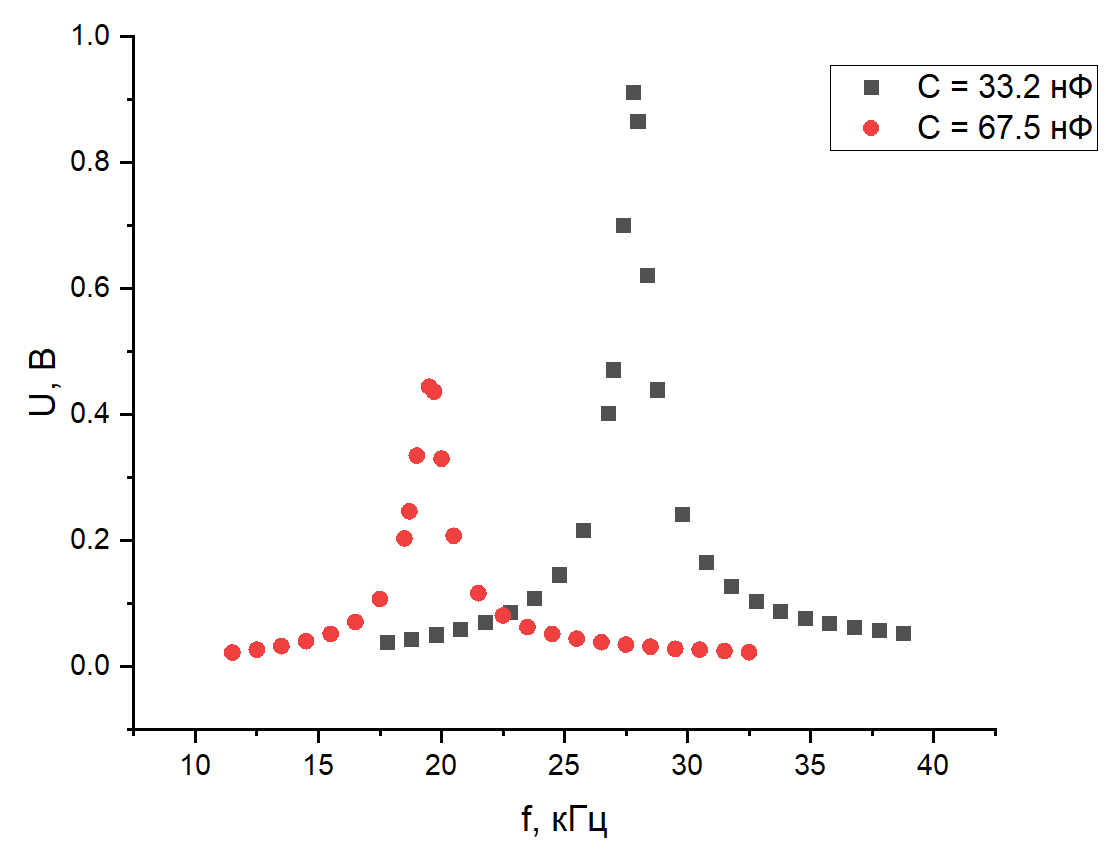
\includegraphics[width=1\linewidth]{ach.png} \\ Рис.2 АЧХ}
	\end{figure}

    \begin{figure}[h!]
        \center{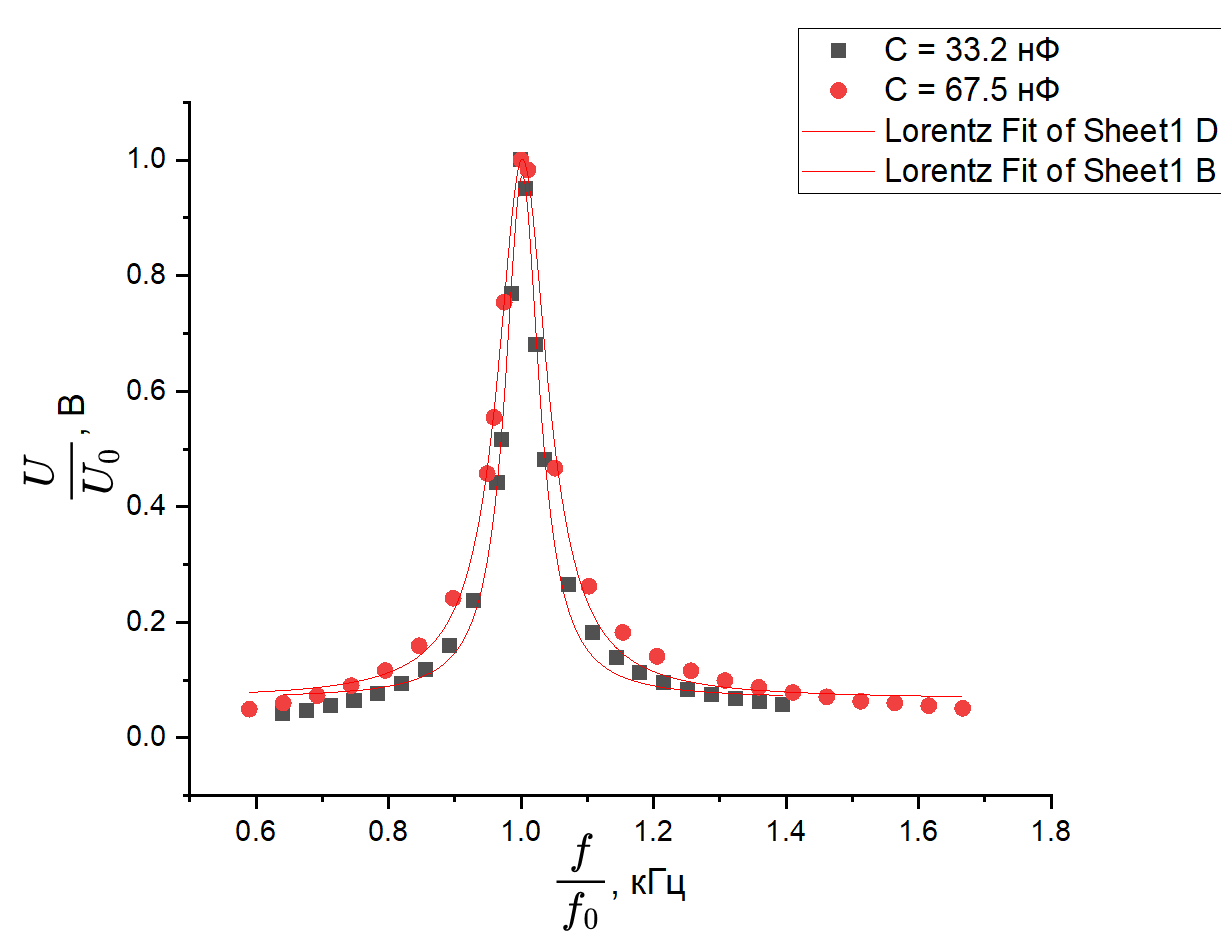
\includegraphics[width=1\linewidth]{ach_norm.png} \\ Рис.2 АЧХ с нормировкой}
        \end{figure}
        \begin{figure}[h!]
            \center{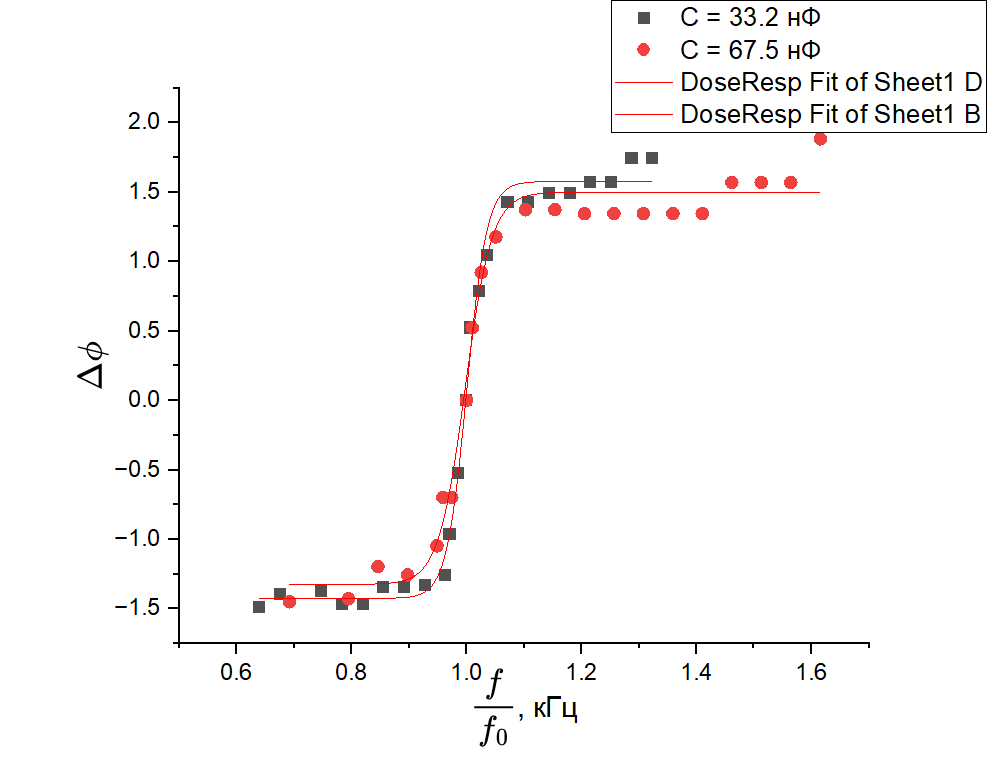
\includegraphics[width=1\linewidth]{fch.png} \\ Рис.2 ФЧХ с нормировкой}
            \end{figure}
        \begin{figure}[h!]
            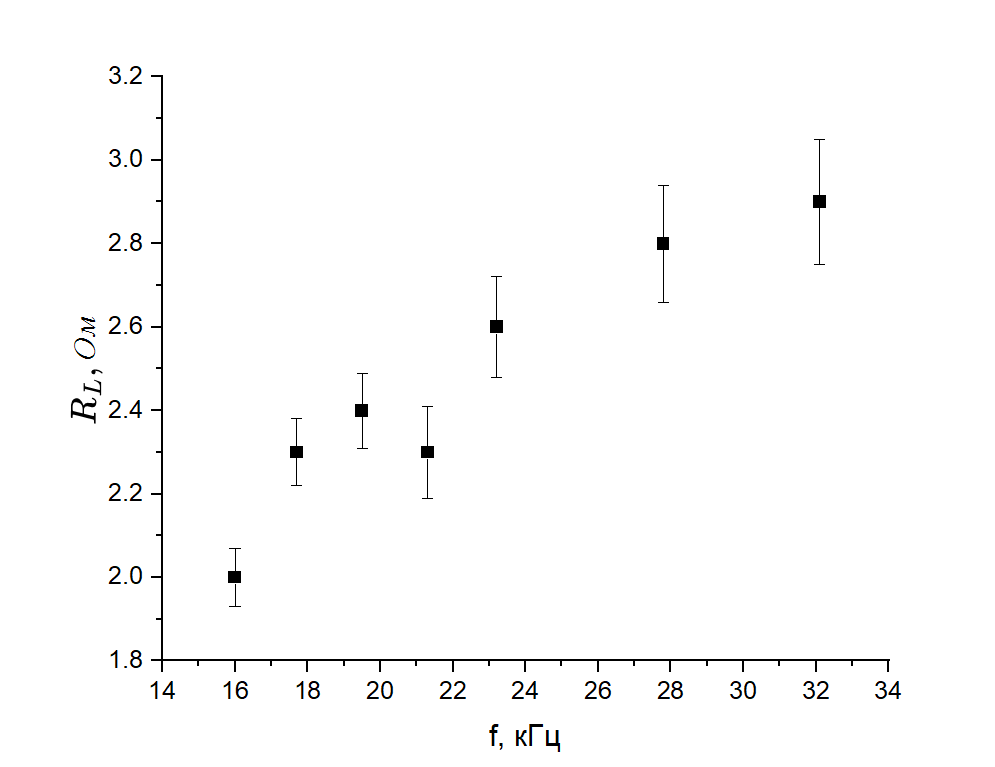
\includegraphics[scale=0.5]{image.png}
            \caption{График зависимости $ R_L (f_{0n}) $}
        \end{figure}
\end{document}